% p2.svg 的 TikZ 矢量源：将第二个置换环反向（左 (2 3)，右 1→4→5→1）
% 编译：latex p2.tex && dvisvgm --exact --no-fonts --precision=8 p2.dvi
\def\pgfsysdriver{pgfsys-dvisvgm.def}
\documentclass[tikz,border=2pt]{standalone}
\usetikzlibrary{arrows.meta}
\pagecolor{white}
\begin{document}
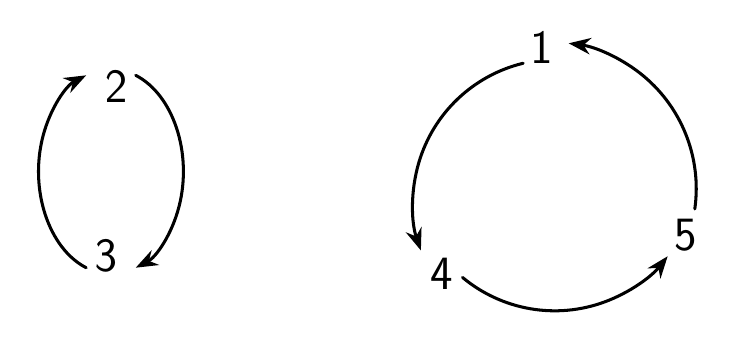
\begin{tikzpicture}[>=Stealth,line width=1.1pt,line cap=round,
  num/.style={font=\LARGE\sffamily,inner sep=1.5pt}]
  % 左环 (2 3)：与 p1 相同
  \node[num] (t) at (3.55,1.0)  {2};
  \node[num] (h) at (3.42,-1.15) {3};
  \begin{scope}[shift={(3.485,-0.075)}]
    \draw[->] (70:0.92 and 1.30) arc[start angle=70,end angle=-70,x radius=0.92,y radius=1.30];
    \draw[->] (250:0.92 and 1.30) arc[start angle=250,end angle=110,x radius=0.92,y radius=1.30];
  \end{scope}
  % 右环：1→4→5→1（与 p1 相同的三段圆弧，反向绘制）
  \node[num] (a) at (8.95,1.5)  {1};
  \node[num] (b) at (10.78,-0.88) {5};
  \node[num] (c) at (7.68,-1.38) {4};
  % 左弧反向（圆心 (9.15,-0.48)，半径 1.83）：1→4
  \draw[->] (8.72,1.30) arc[start angle=103.6,end angle=199.1,radius=1.83];
  % 底弧反向（圆心 (9.12,-0.02)，半径 1.83）：4→5
  \draw[->] (7.95,-1.42) arc[start angle=-129.8,end angle=-38.4,radius=1.83];
  % 右弧反向（圆心 (9.06,-0.29)，半径 1.86）：5→1
  \draw[->] (10.90,-0.55) arc[start angle=-8.0,end angle=82.6,radius=1.86];
\end{tikzpicture}
\end{document}
